%% \chapter[htoc-titlei][hhead-titlei]{htitlei}
%% -----------------------------------------------------------------------------
\chapter[Theoretical overview][Theory]{Theoretical overview}
\label{ch:theory}

{\color{red} I'll need to go back and re-read through some books/papers before
  writing this chapter!}

{\color{red} Evelyn: 
keep this brief by referencing as much as possible.
Certainly contrast assumption of RPC vs assumption of RPV for experimental
searches.
Both are possibilities.
Stop as LSP does give unique (crazy?) signature not well
tested by previous searches (include LQ exclusion plot).
Could have different
decay rates to e, mu, tau.
}

%% ------------------------------------------------------------------------------
\section{Standard Model}

%% ------------------------------------------------------------------------------
\section{Supersymmetry}

Lightest supersymmetric particle (LSP) 

%% - - - - - - - - - - - - - - - - - - - - - - - - - - - - - - - - - - - - - - -
\subsection{R-Parity}

The extension of the Standard Model of particle physics with
supersymmetry (SUSY)~\cite{Miyazawa:1966,Ramond:1971gb,Golfand:1971iw,
Neveu:1971rx,Neveu:1971iv,Gervais:1971ji,Volkov:1973ix,Wess:1973kz,Wess:1974tw}
immediately leads to processes that violate both baryon number ($B$) and
lepton number ($L$), leading to rapid proton decay and
lepton-number-violating processes, such as unseen decays of
$\mu \to e\gamma$, in conflict with experimental bounds.
A conventional assumption to prevent these processes is to impose
conservation of $R$-parity~\cite{Fayet:1976et,Fayet:1977yc,Farrar:1978xj,
Fayet:1979sa,Dimopoulos:1981zb},
defined as $R=(-1)^{3(B-L)+2s}$ where $s$ is the spin of the particle.
This has a value of $+1$ for Standard Model particles and $-1$ for
SUSY particles.
In this case SUSY particles are produced in pairs, and the LSP is stable.
Further, this stable LSP cannot carry electric charge or color charge without
coming into conflict with astrophysical data.
At the LHC, the conventional experimental signature for SUSY particles
includes significant missing transverse momentum due to the non-interaction of
the LSP with the detector.

%% -----------------------------------------------------------------------------
\section{B-L extension}
\label{sec:theory_bl_extension}


%% - - - - - - - - - - - - - - - - - - - - - - - - - - - - - - - - - - - - - - -
\subsection{Motivation}

{\color{red} Why this model? :-) Talk about things like:
\begin{itemize}
\item RPC is overkill to prevent proton decay
\item Links neutrino sector to susy properties
\end{itemize}
}

An alternative approach is to add a local symmetry $U(1)_{B-L}$ to the
$SU(3)_C \times SU(2)_L \times U(1)_Y$ Standard Model with right-handed
neutrinos.
The minimal supersymmetric extension then only needs a vacuum expectation value
for a right-handed sneutrino in order to spontaneously break the
$B-L$ symmetry~\cite{FileviezPerez:2008sx, Barger:2008wn, FileviezPerez:2009gr,
Everett:2009vy, Evans:1986ada, Lukas:1998yy, Braun:2005ux, Braun:2005nv,
Braun:2006ae, Ambroso:2009jd, Ambroso:2010pe, Ovrut:2012wg}.
This minimal $B-L$ model violates lepton number but not baryon number, and is
consistent with proton stability and the bounds on lepton number violation.
The LSP can now decay via $R$-parity-violating (RPV) processes, and may now
carry color and electric charge.

%% - - - - - - - - - - - - - - - - - - - - - - - - - - - - - - - - - - - - - - -
\subsection{Phenomenology}

{\color{red} Why this model? :-)
\begin{itemize}
\item $U(1)_{B-L}$ gauge boson
\item Natural choices for LSP? Why stop
\item relation between stop branching ratios and the neutrino hierarchy)!
\item Why look for $\stop \to b\ell$ instead of
  $\stop \to t\nu$? (handedness argument)
\end{itemize}
}

This leads to unique signatures~\cite{FileviezPerez:2012mj, Perez:2013kla,
Ovrut:2012wg, Ovrut:2014rba, Ovrut:2015uea} that are disallowed in conventional
models with $R$-parity conservation.
The case where the LSP is a scalar top (stop) is most interesting
since, in general, the large mass of the top quark acts to make the
lightest stop significantly lighter than the other squarks due to
renormalization group effects~\cite{Barbieri:1987fn,deCarlos:1993yy}.
The stop decays via an RPV interaction to a charged lepton (of any
flavor) and a $b$-quark.
The decay branching fractions to $e b$, $\mu b$, and $\tau b$ may be different
in a manner related to the neutrino mass
hierarchy as shown in
Figure~\ref{fig:pheno_bounds}.
Each point in this plot represents a simulation with a particular choice of
model parameters, all varied within a natural range of values.
The four colors represent different choices for the neutrino mass hierarchy and 
$\sin^2(\theta_{23})$.
There is a clear relation between the neutrino mass hierarchy and the allowed
stop branching ratios.\cite{Marshall:2014kea, Marshall:2014cwa}

\begin{figure}[ht]
  \centering{
    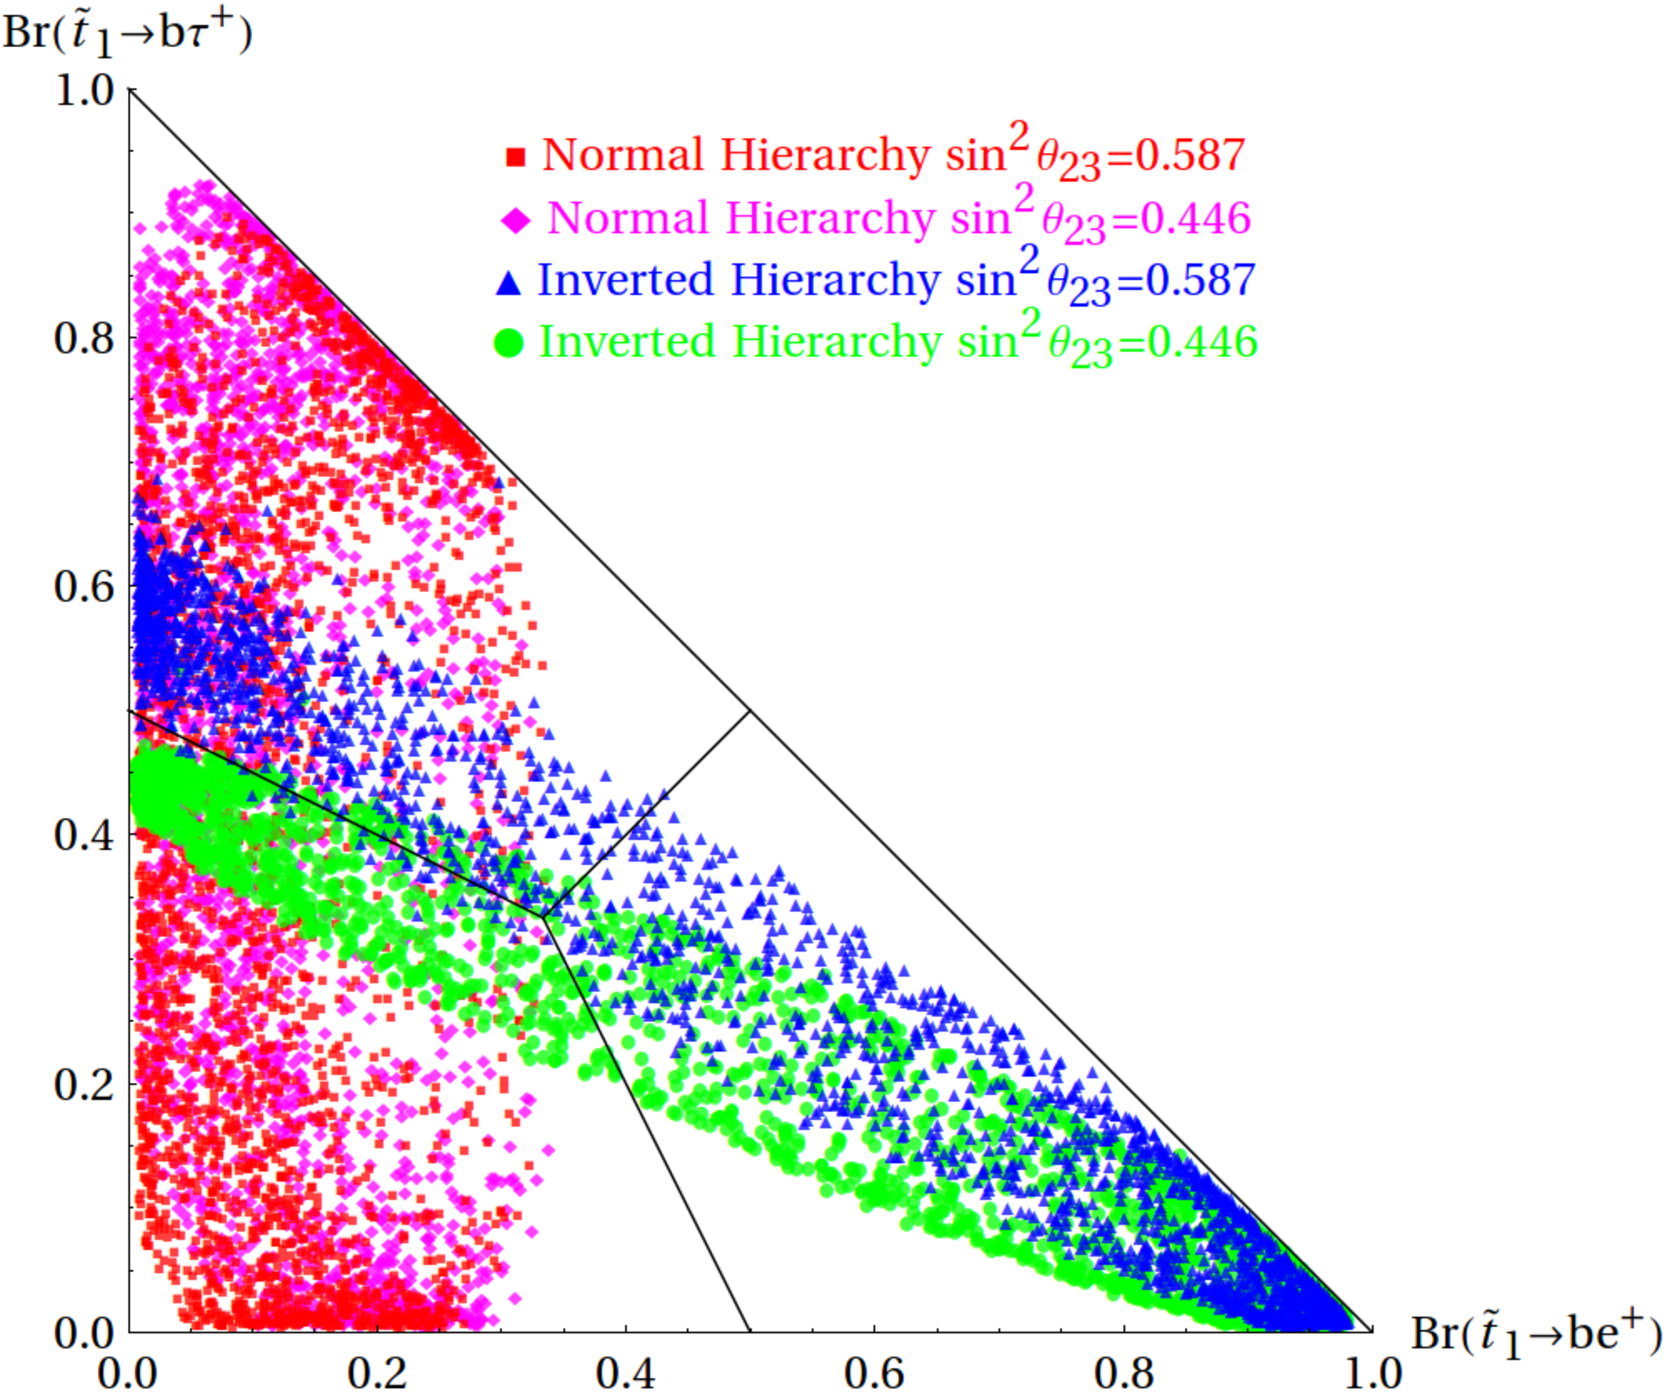
\includegraphics[width=0.75\textwidth]{figs/theory/WithGaussian.pdf}
    \caption{This plot shows the allowed branching ratios for the stop LSP
      for various choices of the neutrino mass hierarchy and
      $\sin^2(\theta_{23})$,
      obtained by varying various model parameters within a range of natural
      values.\cite{Marshall:2014cwa}
    }
    \label{fig:pheno_bounds}
  }
\end{figure}

Within this model, a stop LSP can decay in one of two ways, depending on
the helicity of the stop.
A right-handed stop decays to a top quark and a right-handed neutrino with a
coupling strength proportional to vacuum expectation value (VEV) of the
left-handed neutrino mass.
This must be small because the left-handed sneutrino interacts with the
$W$ and $Z$ bosons, and a large VEV would result in these bosons gaining
additional mass.
{\color{red} (TODO check this statement is true - I think I'm missing
something).}
A left handed stop decays to a $b$-quark and a lepton with the coupling
strength proportional to the VEV of the right-handed sneutrino.
Since the right-handed sneutrino does not couple to the electroweak bosons,
a large VEV does not break electroweak symmetry.
{\color{red} (TODO check this statement is true - I think I'm missing
something)}.
If the stop LSP is an admixture of left- and right-handed stops, the preferred
decay mode depends on the stop mixing angle ($\theta_t$), as seen in
Figure~\ref{fig:stop_br_vs_mixing_angle}, which shows the ratio
$\nicefrac{\mathrm{Br}(\stop \to t\nu)}{\mathrm{Br}(\stop \to b\ell)}$
versus $\theta_t$.
Each point represents a simulation with a particular choice of model parameters.
The $\stop \to b\ell$ decay is the dominant decay mode for mixing
angles less than abut $80^{\circ}$, where the LSP stop is mostly right handed,
and the $\stop \to t\nu$ decay becomes significance.
The $\stop \to b\ell$ decay is still non-negligible for a mostly right-handed
stop in many of the simulated models,
however.\cite{Marshall:2014kea, Marshall:2014cwa}

Since the $\stop \to b\ell$ decay is preferred for most of parameter space,
the analysis described in this thesis will focus on this decay mode.
Additionally, if the $\stop \to t\nu$ decay is significant, the decay of stop
pairs would lead to final states with $t\bar{t}$ associated with large missing
energy.
This is the same final state as stop pair production with $R$-Parity conserving
decays, and the limits from traditional stop searches can be reinterpreted for
this model.

\begin{figure}[ht]
  \centering{
    \subbottom[Stop branching ratio]{
      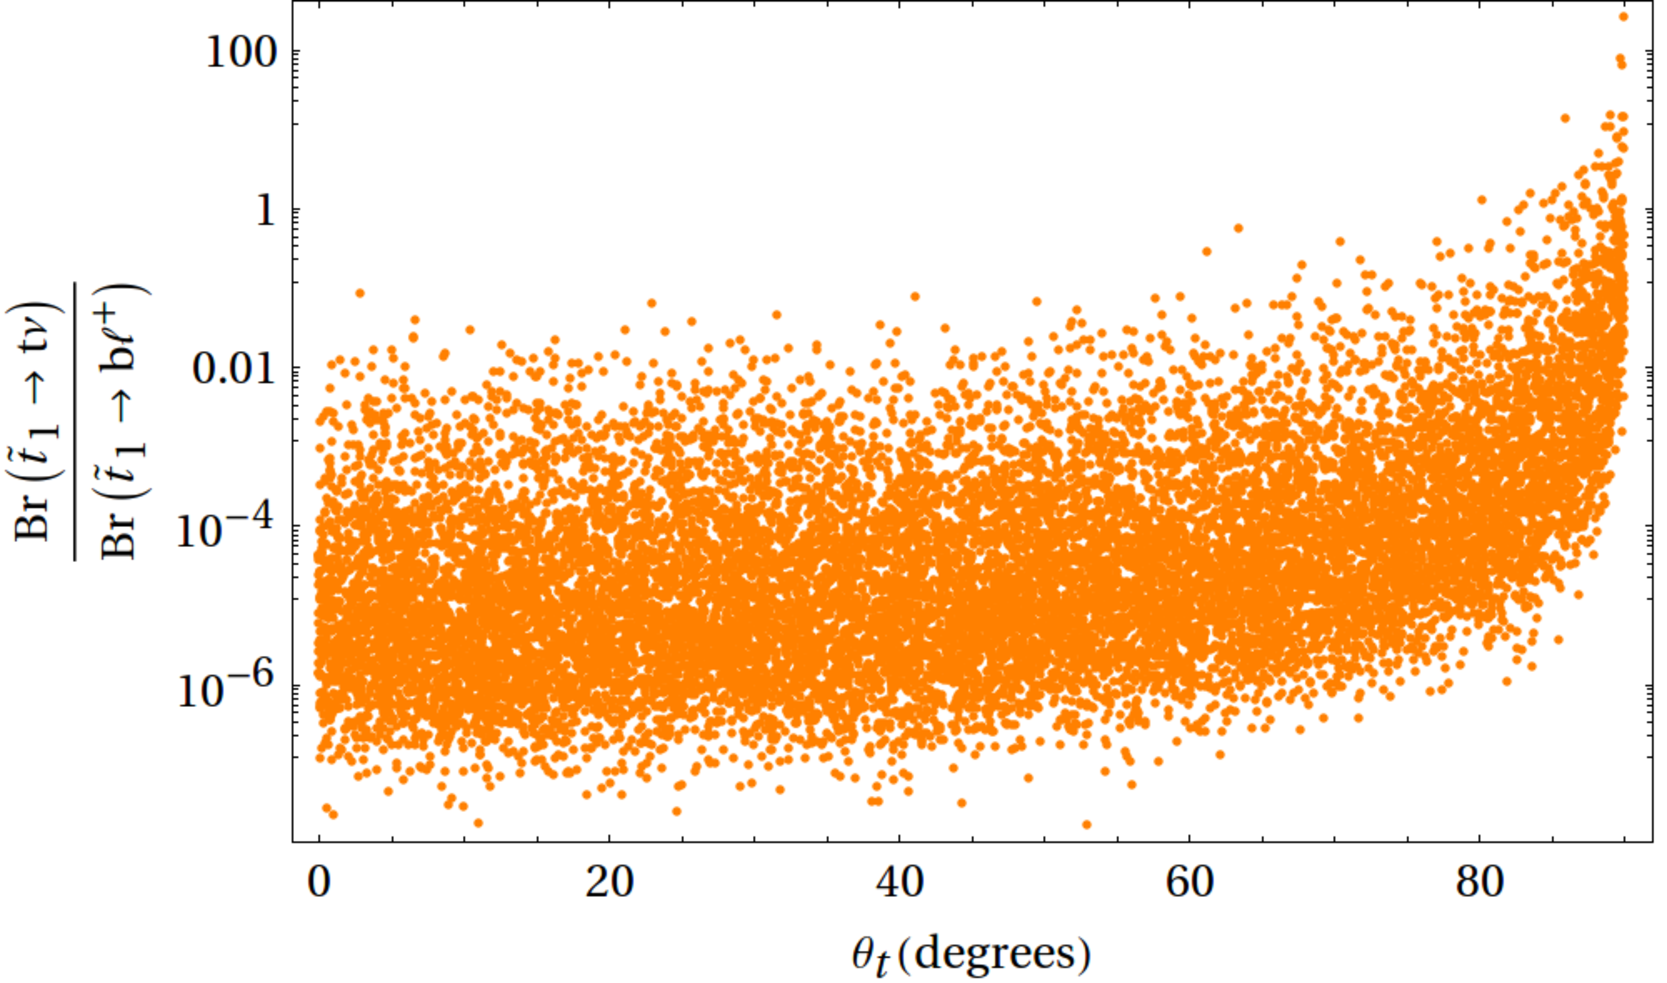
\includegraphics[width=0.45\textwidth]{figs/theory/StopBranchingRatiosVsMixingAngle.pdf}
      \label{fig:stop_br_vs_mixing_angle}
    }
    \subbottom[Stop decay length]{
      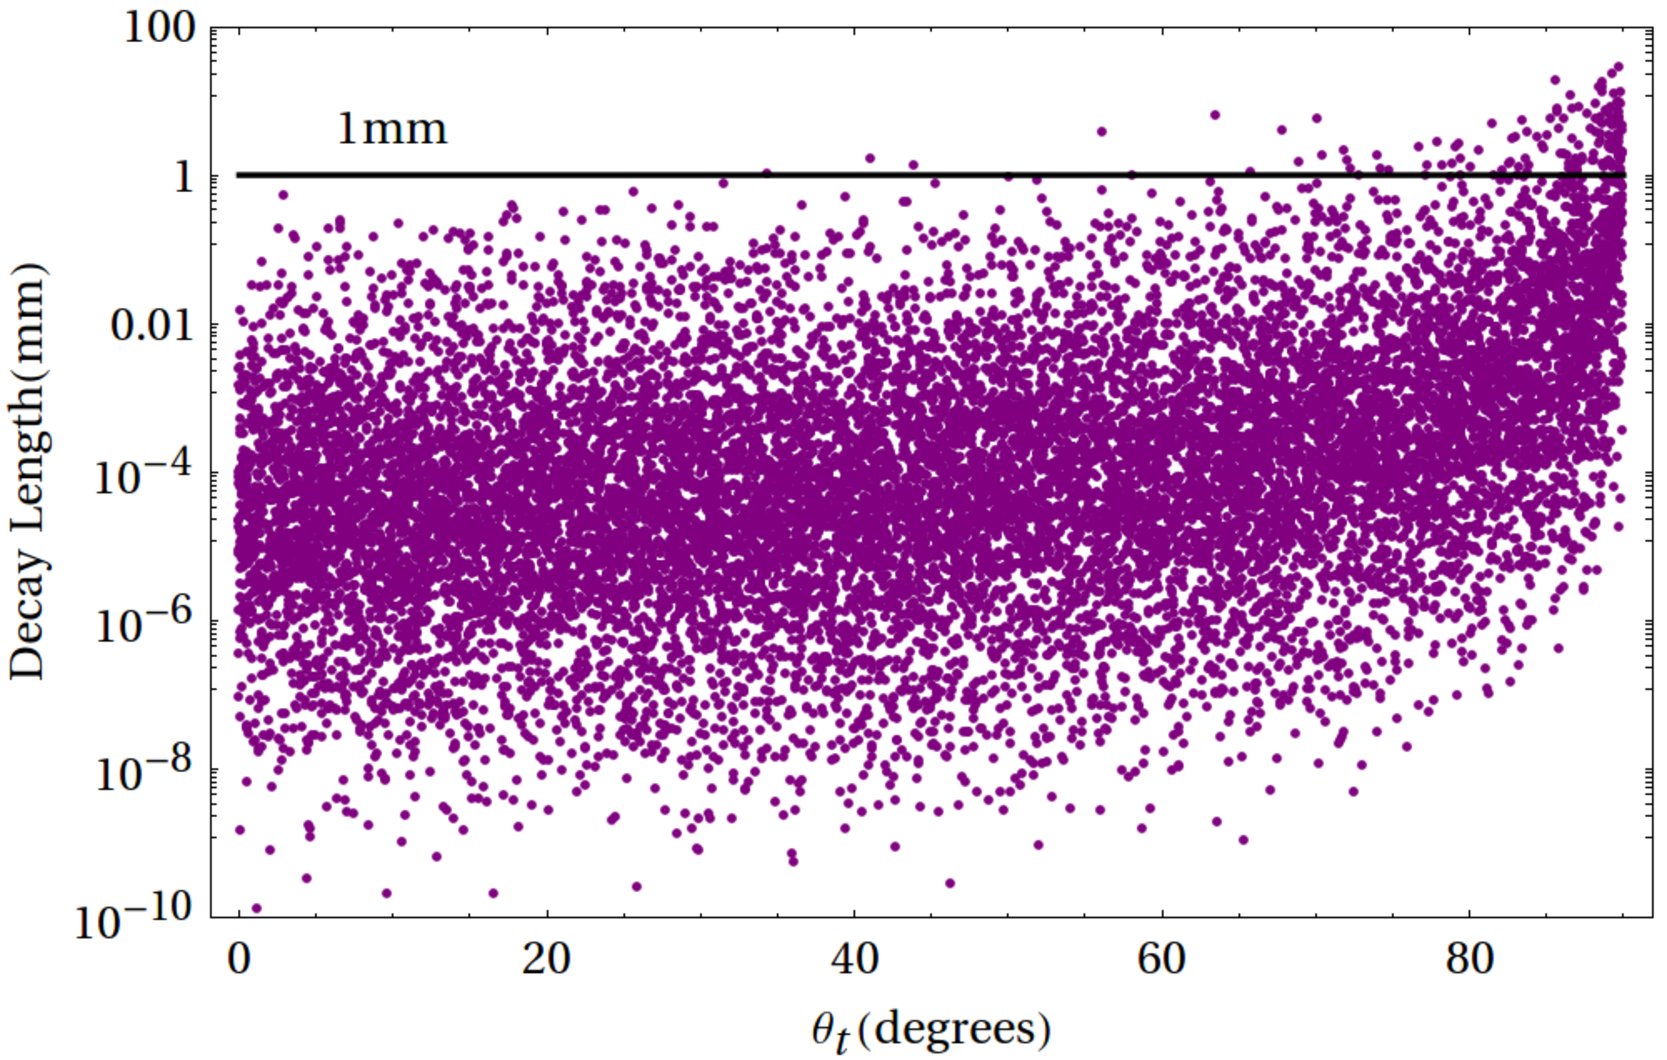
\includegraphics[width=0.45\textwidth]{figs/theory/DecayLength.pdf}
      \label{fig:stop_decay_length_vs_mixing_angle}
    }
    \caption{These plots show the stop decay length and branching ratio versus
      the stop mixing angle, assuming the stop is the
      LSP.
      Each point in these plots represent a simulation with a particular
      choice of model parameters, which are varies within a range of natural
      values.\cite{Marshall:2014cwa}
    }
    \label{fig:stop_vs_mixing_angle}
  }
\end{figure}

\begin{figure}[ht]
  \centering{
    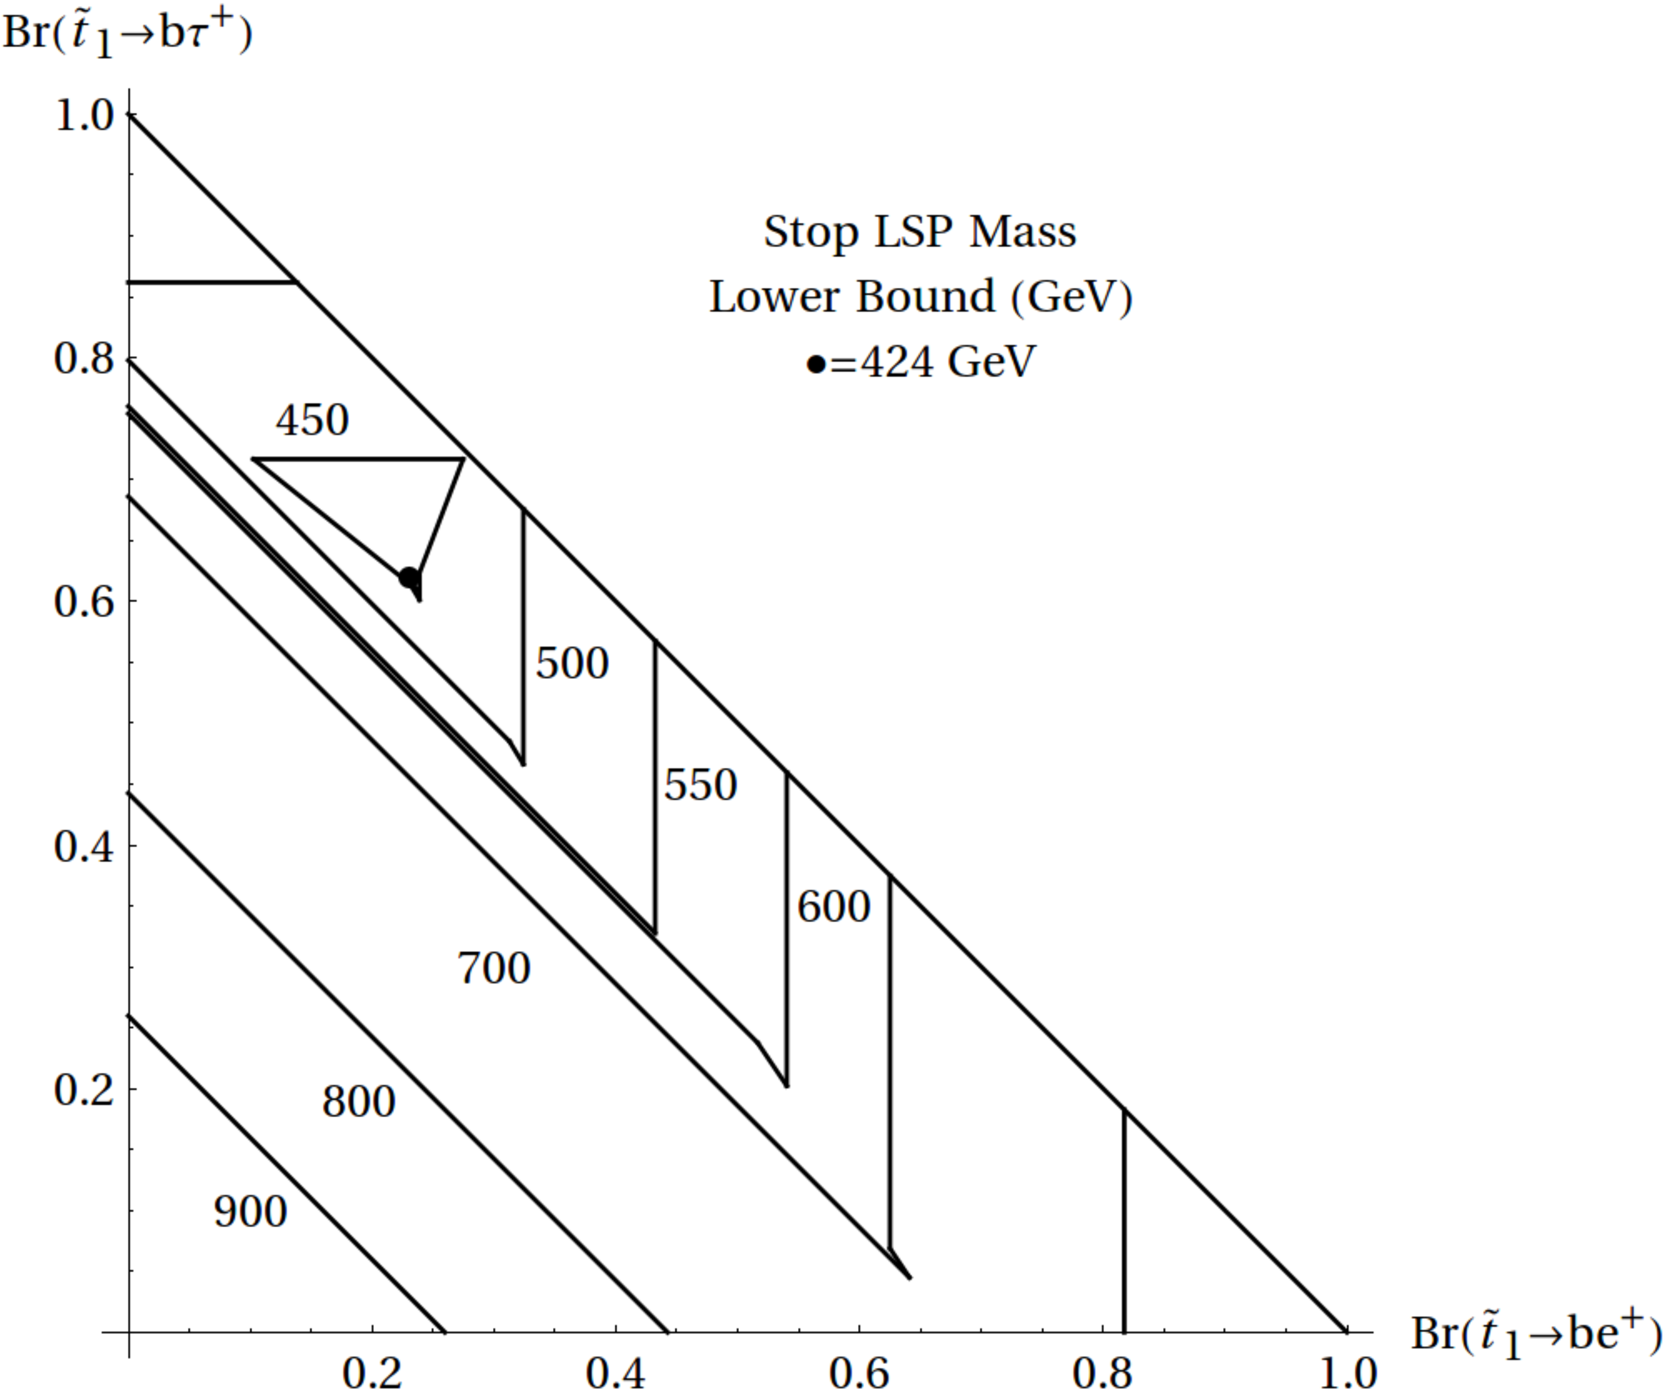
\includegraphics[width=0.75\textwidth]{figs/theory/BoundContourPlotNoCombination.pdf}
    \caption{Limits on the stop mass obtained by reinterpreting lepto-quark
      searches performed at ATLAS.\cite{Marshall:2014cwa}
      The mass limits assume the stop is the LSP, and decays to a $b$-quark
      and a lepton.
    }
    \label{fig:pheno_limit}
  }
\end{figure}

